\chapter{Анализ предметной области}

\section{Ретрансляция видеопотоков}

Ретрансляция видеопотоков --- это повторная передача видеопотоков через компьютерные Сети с целью распространения или обработки.
Ретрансляция начинается с захвата видеопотока с источника, такого как веб-камера, IP-камера, экран компьютера или другое устройство, которое генерирует видеоданные.
Ретрансляция может быть использована для одновременной трансляции видеопотока на несколько устройств, при этом видеопотоки могут подвергаться различным видам обработки: сжатию, кодированию, фильтрации или масштабированию, в зависимости от конкретных потребностей.

\section{Организация ретрансляции видеопотока}

Трансляция формируется надежной системой ретрансляции, в качестве такой системы выступает сервер, который принимает видеопоток от устройства--захвата. Трансляция совершается путем использования протокола, таких как UDP, RTP, RTSP, RTMP и других.
Сетевой протокол в свою очередь должен гарантировать доставку и управление трансляцией, при этом подстраивающийся под условия Сети. Таким образом для передачи  обычно используется один из двух способов.

Последовательный --- видеофайл воспроизводится с жесткого диска сервера провайдера услуг. Как правило, при передаче таким способом качество изображения и звука выше. К недостаткам стоит отнести то, что невозможно переключить ролик с одного момента на другой, не дождавшись его буферизации. То есть, интересующий фрагмент должен быть загружен, чтобы пользователь смог его просмотреть.

В реальном времени --- требует наличия потокового сервера. Этот метод больше подходит для передачи видеофайлов большой длительности. Пользователь может выбрать место, с которого он хочет начать просмотр. Также этот вид потокового передачи мультимедиа используется для трансляции с веб-камеры или захвата экрана.

\section{Модель взаимодействий открытых систем}

Все устройства в компьютерной сети взаимодействую по концептуальной модели взаимодействия открытых систем OSI/ISO. 
Её предложили в 1984 году инженеры из ISO, которая работала над единым стандартом передачи данных по Интернету. 
Модель OSI включает семь уровней, причём каждый из них выполняет определённую функцию и определяется набором протоколов~\cite{tcp_ip_reilly, tcp_ip_lora}.

Модель TCP/IP --- это стек протоколов, которые задают правила передачи данных по Сети. TCP/IP состоит из 4 уровней и покрывает функционал семи уровневой модели OSI/ISO~\cite{tcp_ip_reilly, tcp_ip_lora}.

На рисунке~\ref{pr:protocol} представлено сравнение моделей  OSI/ISO и TCP/IP.

\begin{figure}[h]
	\centering
	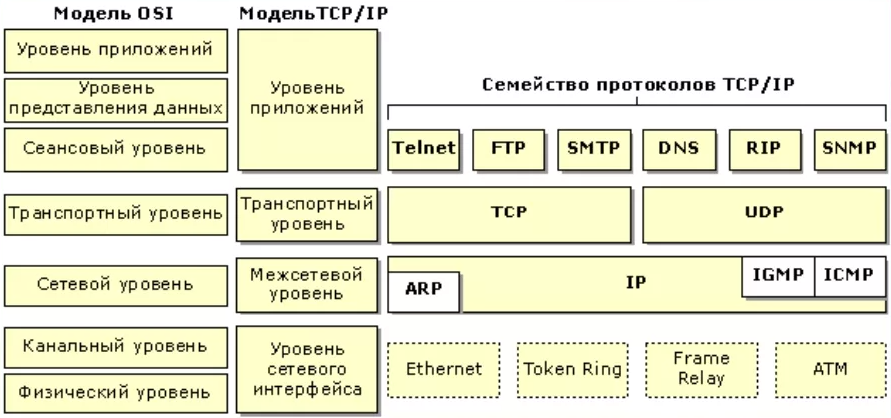
\includegraphics[width=1\textwidth]{img/protocol.png}
	\caption{Модель OSI и TCP/IP~\cite{tcp_ip_reilly, tcp_ip_lora}}
	\label{pr:protocol}
\end{figure}

\clearpage

В таблице~\ref{tab:tcp-ip} представлены уровни TCP/IP.

\begin{table}[ht]
	\begin{center}
		\begin{threeparttable}
			\caption{\label{tab:tcp-ip} Уровни TCP/IP}
			\begin{tabular}{|c|c|>{\arraybackslash}p{9cm}|}
				\hline
				\textbf{Обозначение} & \textbf{Уровень} & \textbf{Назначение} \\ \hline
				L4  	& Прикладной   & Взаимодействие с приложениями и процессами; установление, поддержание и корректного заврешения сеансов соединений, аутентификация; корректное отображение данных. \\ \hline
				L3      & Транспортный &  Обеспечивает надежную доставку данных со сквозным обнаружением и устранением ошибок. \\ \hline
				L2  	& Сетевой	   & Поиск и выбор оптимального машрута между географически удаленными сетями. \\ \hline
				L1    	& Канальный	   & Отвечает за механические, электрические, процедурные и функциональные характеристики установления и завершения соединения между устройствами; отвечает за методы передачи и контроля данных; определяет формат данных для передачи.\\ \hline
			\end{tabular}
		\end{threeparttable}
	\end{center}
\end{table}


\section{Методы передачи информации}

В компьютерных сетях информация передается тремя основными методами: unicast, broadcast и multicast. 
Каждый из трех методов передачи использует различные типы назначения IP--адресов, которые предназначены для конкретных задач и существуют требования, которые необходимо будет поддерживать для каждой из них~\cite{method_streaming}.

Broadcast или широковещательная передача пакетов --- процесс передачи, при котором информация отправляется одним узлом и доставляется всем узлам в сети с использованием специального IP--адреса. В таком случае все клиенты получат информацию без необходимости запрашивать ее, поэтому данный метод используется лишь для передачи служебной информации~\cite{method_streaming, differece_method_streaming_2}.

Unicast или одноадресная рассылка --- процесс передачи, при котором информация отправляется от одного отправителя к одному получателю. Каждый получатель запрашивает персональный видео-контент в произвольное и удобное ему время.
Число таких клиентов может быть ограничено лишь пропускной способности и скорости сети~\cite{method_streaming}.

Multicast или многоадресная рассылка --- процесс передачи, при котором информация отправляется от одного отправителя к нескольким выбранным получателям, находящихся в группе в частной сети.  Multicast использует специальный класс IP--адресов назначения, при этом каждый адрес привязан к группе получателей. Данный метод был разработан для того, чтобы не нагружать Сеть, путем отправки пакета выбранной группе получателей~\cite{method_streaming}. 

Таким образом, для передачи видеопотоков используются unicast или multicast. Multicast отлично подходит для внутренней потоковой передачи в частных сетях, в то время как unicast является лучшим вариантом для передачи в общедоступной сети, поскольку она не предполагает специализированной и ручной настройки Сети~\cite{differece_method_streaming_1}.

\chapter{Обзор существующих решений}

Согласно общепринятым нормам взаимодействия открытых систем, передачей данных между сервером и клиентом регламентируется протоколами транспортного уровня, на котором выполняется сегментация данных от отправителя и организацию потока на получателе~\cite{tcp_ip_reilly,  network_tanenbaum}. 

Вместе с этим решаются задачи:
\begin{itemize}
	\item мультиплексирование;
	\item установление и управление соединение;
	\item управление потоком;
	\item надежность передачи данных.
\end{itemize}

Таким образом, протоколы прикладного и транспортного уровня для передачи видеопотоков реализованы поверх двух важных протоколов транспортного уровня --- TCP и UDP.

\section{TCP}

TCP --- протокол с установлением соединения, обеспечивающий надежную доставку данных со сквозным обнаружением и устранением ошибок.
Надежность в TCP обеспечивается благодаря механизму подтверждения приема повторной передачей PAR, в случае его потери или искажения. Согласно TCP гарантируетcя доставка данных и соединение ложно установиться до начала передачи данных, путем <<тройного рукопожатия>>. По такому же принципу происходит разъединение соединения~\cite{tcp_ip_reilly, tcp_ip_lora}. 

\clearpage

На рисунках~\ref{pr:conn_network} предствлены процессы соединения и разъединения между сервером и клиентом.

\begin{figure}[h]
	\centering
	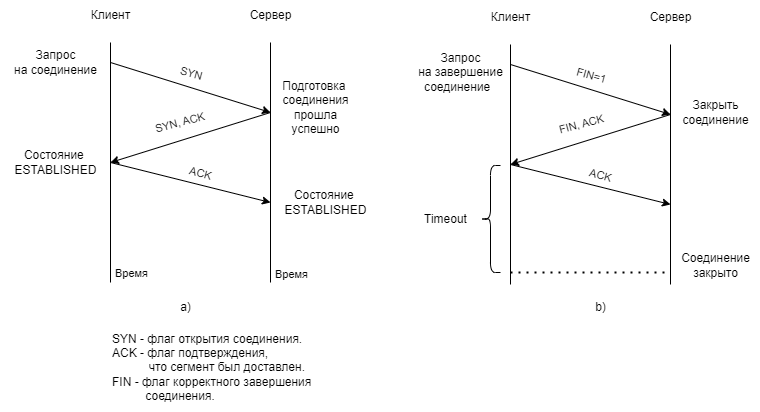
\includegraphics[width=1\textwidth]{img/tcp_network.png}
	\caption{Схема процессов соединение (а) и разъединение (b)~\cite{tcp_ip_reilly}}
	\label{pr:conn_network}
\end{figure}

Также TCP регулирует скорость отправки в соответствии со своей оценкой пропускной способности Сети, потери и задержку, и если они ухудшились, это снизит скорость потока, а если они улучшились, это увеличит скорость потока. 
В случае потери пакета во время передачи, пакет передается  повторно~\cite{tcp_ip_reilly, tcp_ip_lora, protocls_lakin}. 

TCP использует метрики, собираемые в процессе работы протокола, чтобы определить дальнейшую взаимодействие. Из полученных метрик высчитывается размер TCP-окна, показывающий количество байт, которые принимающая сторона готова принять в текущий момент без подтверждения~\cite{tcp_ip_reilly}.

RTT (Round-Trip Time) необходимое время для отправки данных клиенту и обратно, которое включает время задежки на передачу данных и подтверждения получения пакета. У RTT есть отклонение --- devRTT (deviation of Round-Trip Time).
DevRTT и среднее RTT используются для управления потоком, определения промежутка времени, после которого пакеты будут считаться утерянными~\cite{rfc_tcp}.

RTT рассчитывается по следующей формуле:
\begin{equation*}
	\label{formula:rtt}
	RTT_i = t_{r} - t_{0},
\end{equation*}
где $t_{r}$ --- время получения подтверждения пакета, $t_{0}$ --- время отправки пакета, $RTT_i$ --- RTT i-ого пакета.

Cреднее значение RTT рассчитывается по следующей формуле:
\begin{equation*}
	\label{formula:avg_rtt}
	RTT_{average} = \alpha RTT_{average} - \beta RTT_{i},
\end{equation*}
где $\alpha = 0,875$  и $\beta = 0,125$.

Отклонение RTT рассчитывается по следующей формуле:
\begin{equation*}
	\label{formula:dev_rtt}
	DevRTT_{i} = |RTT_{i} - RTT_{average}|,
\end{equation*}

Среднее отклонение RTT рассчитывается по формуле: 
\begin{equation*}
	\label{formula:avg_dev_rtt}
	DevRTT_{average} = \alpha DevRTT_{average} - \beta DevRTT_{i},
\end{equation*}
где $\alpha = 0,75$  и $\beta = 0,25$.

Timeout рассчитывается по следующей формуле:
\begin{equation*}
	\label{formula:timeout}
	timeout = RTT_{average} - 4DevRTT_{average},
\end{equation*}

\section{UDP}

UDP --- протокол без установления соединения.
Поскольку протокол UDP таких проверок не совершает и нет механизма PAR, что обеспечивает более быструю передачу данных, но не предоставляет надежность их передачи.

\clearpage

UDP выполняет три действия:
\begin{itemize}
	\item идентифицирует процесс отправки и получения, используя номера портов;
	\item запускает проверку на ошибку в заголовке;
	\item записывает проверку в заголовке.
\end{itemize}
Поэтому UDP не восстанавливает потерянные пакеты~\cite{tcp_ip_reilly, tcp_ip_lora, protocls_lakin}. 

Таким образом, UDP применяется для передачи видеопотоков в реальном времени, потеря пакета данных не приведет к задержке видео для восстановления пакета, но при этом качество видео будет ухудшаться в зависимости от того, сколько пакетов было потеряно.

Для передачи видеопотоков используются протоколы транспортного уровня без установления соединения. 
Так как UDP не может гарантировать качество видео при потере последовательности пакетов, то его используют в сочетании с специальными протоколами, которые преобразуют исходные данные таким образом, что они могут быть переданы в сеть, как непрерывная последовательность, обеспечивается наилучшая потоковую передачу видео, чем TCP. Использование передовых технологий сжатия и буферизации  позволяет просматривать потоковый контент с любого места, не дожидаясь его полной загрузки на компьютер пользователя. 
При этом протоколы формируют полезную нагрузку пакетов, включая необходимые поля и данные~\cite{basic_stream_protocls}. 

\section{MPTCP}

MPTCP~\cite{rfc-mptcp-6824} --- протокол транспортного уровня, использующий несколько каналов передачи данных, который является набором расширений к протоколу TCP, разработанный IETF в 2013 году.

Протокол использует обратное мультиплексирование, разбивая один \newline MPTCP--поток на несколько TCP--потоков, каждый из которых проходит через отдельных канал передачи данных и имеет отдельный идентификатор. Каждый TCP--поток может использовать разные пути для передачи данных. 
На устройстве клиента MPTCP собирает все TCP--потоки в MPTCP--поток, т.е. в единую последовательность.
MPTCP обеспечивает контроль за передачей данных, адаптируясь к пропускной способности Сети.
К примеру, если один из путей недоступен или обладает плохим качеством связи, то автоматически переключается на другой путь.
Таким образом, MPTCP поддерживает беспроводные сети, где качество соединений может меняться в зависимости от местности и времени~\cite{rfc-mptcp-6824, rfc-mptcp-8684}. 

MPTCP может использовать все доступные сетевые интерфейсы для передачи данных одновременно и балансировать нагрузки между интерфейсами, что позволяет достичь увеличение пропускной способности и уменьшение задержки, так как данные могут быть переданы по самому быстрому каналу.
Однако, внедрение MPTCP требует поддержки со стороны устройств, настройки и управления соединением.

\section{RTP}

RTP~\cite{rtp_rtcp_overview} --- прикладной протокол сквозной доставки данных в режиме реального времени, включая видео и аудио.
RTP  позволяет компенсировать негативное влияние задержек на качество видео и аудио, но при этом не гарантирует своевременную доставку пакетов, т.е. не обеспечивает QoS. Также не предоставляет функции исправления ошибок и управления потоком.
RTP совместно используется c UDP используя его функции. 
RTP предусматривает индикацию типа полезной нагрузки
и порядкового номера пакета в потоке, а также применение временных
меток. Отправитель помечает каждый RTP-пакет временной меткой,
получатель извлекает ее и вычисляет суммарную задержку. Разница в
задержке разных пакетов позволяет определить джиттер и смягчить его
влияние --- все пакеты будут выдаваться приложению с одинаковой
задержкой~\cite{rtp_rtcp_overview, rtp_rtcp_ip_telefone, rtp_rtcp_rtsp_mc}.

Однако RTP может использоваться c TCP. 
Также RTP поддерживает передачу данных нескольким адресатам с использованием многоадресной рассылки, если это предусмотрено базовой сетью~\cite{rtp_rtcp_overview}.

На рисунке~\ref{pr:rtp_udp} представлена схема передачи пакета между клиентом и сервером по протоколу RTP поверх UDP.

\begin{figure}[h]
	\centering
	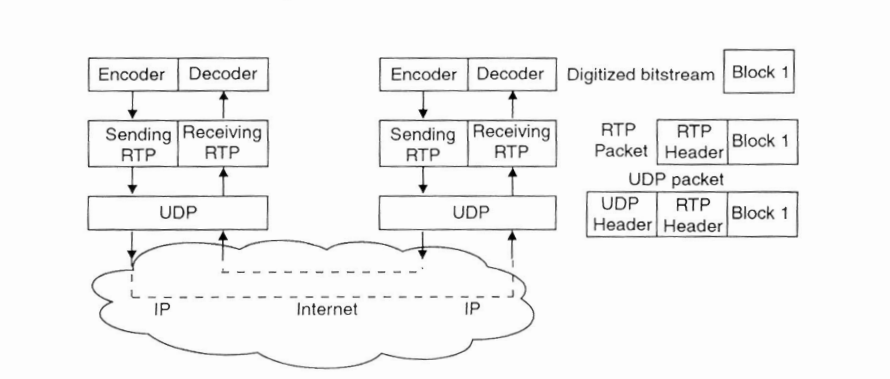
\includegraphics[width=0.8\textwidth]{img/rtp_over_udp.png}
	\caption{Схема  передачи пакета между клиентом и сервером по RTP поверх UDP~\cite{rtp_rtcp_rtsp_mc}}
	\label{pr:rtp_udp}
\end{figure}

\section{RTCP}

RTCP~\cite{rtp_rtcp_overview} --- протокол управления, созданный для совместной работы с RTP, он помогает осуществлять синхронизацию видео и звука, обеспечивать QoS, т.е. обратную связь участников сеанса RTP и контроль качества передачи данных. Также RTCP передает сведения о числе переданных и потерянных пакетов, значения джиттера, задержке и т.д.
Базовый протокол должен обеспечивать мультиплексирование пакетов данных и управления, в UDP это обычно реализуется с использованием отдельных номеров портов.

Основными функциями RTCP являются:
\begin{itemize}
	\item мониторинг качества обслуживания и контроль перегрузки;
	\item идентификация источника RTP;
	\item оценка размера сеанса и масштабирование.
\end{itemize}
Пакеты RTCP содержат прямую информацию для мониторинга качества обслуживания. 
Отчеты отправителя (SR) и отчеты получателя (RR) обмениваются информацией о потерях пакетов, задержке и джиттера. 
Эта информация может быть использована для реализации механизма управления потоком, подобного TCP.
Средство управления сетью может отслеживать загрузку Сети на основе пакетов RTCP без получения фактических данных или обнаруживать неисправные участки Сети~\cite{rtp_rtcp_overview, rtp_rtcp_rtsp_mc}.
 
На рисунке~\ref{pr:rtcp_udp} представлена схема передачи пакета между клиентом и сервером по протоколу RTCP.

\begin{figure}[h]
	\centering
	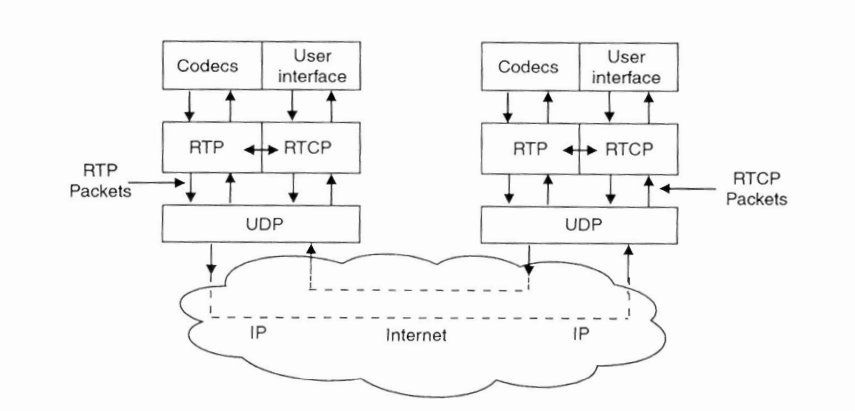
\includegraphics[width=0.67\textwidth]{img/rtcp_over_udp.png}
	\caption{Схема передачи пакета между клиентом и сервером по RTCP~\cite{rtp_rtcp_rtsp_mc}}
	\label{pr:rtcp_udp}
\end{figure}

\section{RTSP}

RTSP~\cite{rfc_rtsp} --- протокол управления прикладного уровня для инициализации и направления потоковых данных от видеосервера, реализующий возможности «удаленного управления», который был разработан в 1996 году для управления развлекательными и коммуникационными системами видеотрансляций.

RTSP требует двух типов компонентов для успешного выполнения потоковой передачи --- клиента и сервера. Сервер обслуживает потоковые данные, а клиент запрашивает их. отдельного сервера для приема запросов от нескольких клиентов и потоковой передачи данных, который поддерживает сеанс RTSP постоянного соединения с клиентами RTSP, помеченный идентификатор, при этом во время соединения сеанс не привязывается к использованию транспортного протокола, поскольку он реализует надежность на прикладном уровне. RTSP не навязывает использования определенного формата медиафайлов.
Во время сеанса, клиент RTSP может открывать и закрывать множество надежных транспортных подключений к серверу для выдачи запросов RTSP. 
Таким образом, могут передаваться несколькими различными способами~\cite{rfc_rtsp}:
\begin{itemize}
	\item постоянные транспортные соединения, используемые для нескольких транзакций запрос--ответ;
	\item одно подключение на транзакцию запроса--ответа;
	\item режим без установления соединения. 
\end{itemize}

RTSP управляет потоком, который может быть отправлен по отдельному протоколу, независимому от канала управления.
Так RTSP используется TCP для передачи и приема команд управления, в то время как данные передаются по UDP. При этом RTSP использует RTP и RTCP для передачи потоков в реальном времени, что в свою очередь обеспечивает воспроизведение RTSP-потока во время загрузки потока и получение потока продолжается если сервер не получает запросов, что называется сегментация потока передачи данных. 
Кроме того, в течение всего срока службы один медиапоток может управляться запросами RTSP, выдаваемыми последовательно по разным TCP-соединениям, поэтому сервис поддерживать <<состояние сеанса>>, чтобы сопоставлять запросы с потоком~\cite{rfc_rtsp}. 

RTSP не конкретизируется на формате передачи данных, поэтому позволяет клиенту выбрать подходящую комбинацию видеоданных, но поддержка кодеков ограничена, что может ограничивать качество видео. У RTSP передается поток с минимальной задежкой, которая достигается до 2 секунд.
Каждый поток идентифицируется по URL-адресу RTSP, который указывает на сервер обрабатывающий этот поток.

\clearpage 

Помимо параметров видео, необходимо определять сетевой адрес назначения и порт, что выделяет несколько режимов работы~\cite{rfc_rtsp}:
\begin{itemize}
	\item многоадресная рассылка и сервер выбирает адрес;
	\item многоадресная рассылка и клиент выбирает адрес;
	\item одноадресная рассылка.
\end{itemize}

На рисунке~\ref{pr:rtsp} представлена схема передачи видеопотока между серверами и клиентом по протоколу RTSP.

\begin{figure}[h]
	\centering
	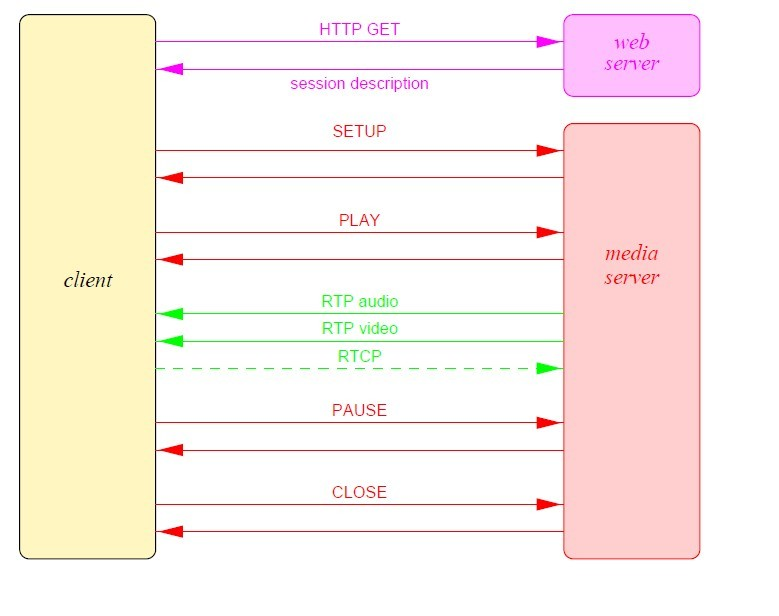
\includegraphics[width=0.8\textwidth]{img/rtsp.jpeg}
	\caption{Схема передачи видеопотока между серверами и клиентом по протоколу RTSP}
	\label{pr:rtsp}
\end{figure}

\clearpage

Основные методы протокола, который идентифицируется по запросу:
\begin{itemize}
	\item DESCRIBE --- запрос описания содержимого, например, в формате SDP;
	\item OPTIONS --- запрос поддерживаемых методов;
	\item PLAY --- запрос начала вещания содержимого;
	\item PAUSE --- запрос временной остановки вещания;
	\item RECORD --- запрос на записывание содержимого сервером;
	\item REDIRECT --- запрос на перенаправление на другое содержимое;
	\item SETUP --- запрос установки транспортного механизма для содержимого;
	\item ANNOUNCE --- запрос на обновление данных описания содержимого;
	\item TEARDOWN --- запрос на остановку потока и освобождение ресурсов.
\end{itemize}

По функциональности RTSP совпадает с НTTP и может взаимодействовать с ним, только если первоначально взаимодействие с потоком осуществляется через веб--страницу с помощью специального программного обеспечения.
Однако RTSP принципиально отличается от HTTP тем, что доставка данных осуществляется вне диапазона по другому протоколу, но для работы с кэшами, прокси-серверами и аутентификацией используется аналогичный  функционал HTTP. Таким образом RTSP несовместим с HTTP. Также RTSP  требует большей пропускной способности, что делает его менее подходящим для мобильных устройств~\cite{rfc_rtsp, rfc_http_auth}.

\section{RTMP}

RTMP~\cite{rtmp_adobe} ---  проприетарный протокол прикладного уровня, разработанный Adobe в 2009 году, для высокоэффективной потоковой передачи видео в реальном времени через Интернет между Adobe Flash и сервером.
RTMP предоставляет двустороннюю многоканальную службу передачи сообщений с использованием надёжного транспортного потока путем использования протокола TCP, используемого для передачи параллельных потоков видео, аудио и текстовых сообщений с второстепенной тактовой информацией между парой общающихся пользователей.
Различные классы сообщений получают разные приоритеты, что влияет на их очерёдность в транспортном потоке, когда пропускная способность ограничена.

RTMP нацелена на обеспечение стабильной и плавной передачи увеличивающихся объемов данных, необходимых для передачи и приема видео в реальном времени, что достигается посредством сегментации потока данных на небольшие одинаковые части (аудио --- 64 байта, видео --- 128 байтов), их последовательную передачу через постоянное TCP-соединение на принимающее устройство, которое затем снова собирает их в видеопоток. 
Для трансляции c устройства-источника  видеопоток передается сервер кодировщик, данный этап называется <<первой милей>>. 
Затем сервер обрабатывает поток и передает его дальше для ретрансляции на устройства клиентов, этап называется <<последняя миля>>.
С этого момента поток перехватывается поток другой связи (HLS, MPEG-DASH или WebRTC) или Adobe Flash~\cite{rtmp_adobe}.

Таким образом постоянное соединение обеспечивает надежность доставки видеопотока, которое не отключается при нестабильной передачи данных между сервисом и клиентом, что обеспечивает низкую задержку передачи данных до 5 секунд. 
Благодаря постоянному соединению клиент может подключаться к и отключаться от трансляции, перематывать ее, но оно трудно поддерживается в определенных условиях Сети.
У RTMP низкая пропуская способность, что может стать причиной потери пакетов без восстановления, что может ухудшить качетсво видео.
RTMP протокол не поддерживает HTML5-плеерами и не совместим с HTTP. Поскольку он требует аутентификации, RTMP является гораздо более безопасным протоколом потоковой передачи.~\cite{rtmp_adobe}.

\chapter{Сравнение существующих решений}

В качестве критерий сравнение протоколов для организации ретрансляции видеопотоков необходимо наличие тех или иных возможностей:
\begin{enumerate}
	\item метод передачи потока;
	\item проприетарность;
	\item установка соединения;
	\item гарантированная доставка;
	\item упорядоченная передача --- данные доставляются в том порядке, в котором были отправлены;
	\item поддержка нескольких интерфейсов;
	\item зависимость --- протокол реализован таким образом, что работает поверх нижележащих протоколов;
	\item задержка;
	\item многопоточность;
	\item управление и контроль потоком.
\end{enumerate}

В таблицах~\ref{tab:comparison_1}--\ref{tab:comparison_2} представлено сравнение рассмотренных протоколов для организации передачи видеопотоков.

\clearpage

\begin{sidewaystable}
	\centering
	\begin{threeparttable}
		\caption{\label{tab:comparison_2} Сравнение рассмотренных протоколов (Часть 1)}
		\begin{tabular}{|>{\centering\arraybackslash}p{2.5cm}|>{\centering\arraybackslash}p{2cm}|>{\centering\arraybackslash}p{1cm}|>{\centering\arraybackslash}p{2.5cm}|>{\centering\arraybackslash}p{3.5cm}|>{\centering\arraybackslash}p{1cm}|>{\centering\arraybackslash}p{1cm}|>{\centering\arraybackslash}p{1.5cm}|>{\centering\arraybackslash}p{2cm}|>{\centering\arraybackslash}p{1cm}|>{\centering\arraybackslash}p{3cm}|}
			\hline
			\multirow{2}{*}{\textbf{Протокол}} & \multicolumn{10}{c|}{\textbf{Номер критерия}} \\ \cline{2-11}
			& \textbf{1}   & \textbf{2} 	   & \textbf{3} & \textbf{4} & \textbf{5} & \textbf{6} & \textbf{7} & \textbf{8} & \textbf{9} & \textbf{10} \\ \hline
			\textbf{TCP}       & Unicast  & Нет & <<Тройное рукопожатие>> & Механизмы подтверждения, повторной передачи и контроля порядка пакетов & Да & Нет & Нет & от 100 мс. & Нет & TCP-окна \\ \hline
			\textbf{UDP}  	   & Unicast  & Нет & Нет					   & Нет & Нет & Нет & Нет      & от 1 мс. & Нет & Нет \\ \hline
			\textbf{MPTCP}     & Unicast  & Нет & <<Тройное рукопожатие>> & Да  & Да  & Да  & TCP      & 30-100 мс. & Да & Использует несколько путей для передачи данных \\ \hline
			\textbf{RTP}  	   & Multicast & Нет & Нет                     & Нет & Нет & Нет & TCP/ UDP & от 10 мс. & Да & Контроль битрейта \\ \hline
			
		\end{tabular}
	\end{threeparttable}
\end{sidewaystable}

\clearpage

\begin{sidewaystable}
	\centering
	\begin{threeparttable}
		\caption{\label{tab:comparison_1} Сравнение рассмотренных протоколов (Часть 2)}
		\begin{tabular}{|>{\centering\arraybackslash}p{2.5cm}|>{\centering\arraybackslash}p{2cm}|>{\centering\arraybackslash}p{1cm}|>{\centering\arraybackslash}p{2.5cm}|>{\centering\arraybackslash}p{2cm}|>{\centering\arraybackslash}p{2cm}|>{\centering\arraybackslash}p{1cm}|>{\centering\arraybackslash}p{1.5cm}|>{\centering\arraybackslash}p{2cm}|>{\centering\arraybackslash}p{1cm}|>{\centering\arraybackslash}p{3.5cm}|}
			\hline
			\multirow{2}{*}{\textbf{Протокол}}& \multicolumn{10}{c|}{\textbf{Номер критерия}} \\ \cline{2-11}
			& \textbf{1}   & \textbf{2} 	   & \textbf{3} & \textbf{4} & \textbf{5} & \textbf{6} & \textbf{7} & \textbf{8} & \textbf{9} & \textbf{10} \\ \hline
			\textbf{RTCP}      & Multicast & Нет & Нет                     & Нет & Нет & Нет & RTP & от 10 мс. & Да & Сбор информации о качестве передачи данных, cинхронизация участников и управления параметрами потока данных \\ \hline
			\textbf{RTSP}  	   & Multicast & Нет & Постоянное соединение & Функции TCP & Функции TCP & Нет & RTP/ TCP/ UDP & 2 c. & Да &  Управление воспроизведением, паузой, перемоткой и другими параметрами потока \\ \hline
			\textbf{RTMP}  	   & Unicast   & Да & Постоянное соединение & Функции TCP & Функции TCP & Нет & TCP & 5 c. & Да & Контроль битрейта и параметров передачи потока \\ \hline
		\end{tabular}
	\end{threeparttable}
\end{sidewaystable}

\clearpage

Протокол UDP обладает ограниченным набором действий, на основе которого можно будет реализовать свой протокол для передачи видеопотока. Как было уже сказано TCP в Сети не используется для передачи видеопотоков из-за высокой задержки, хотя присутствуют TCP-окна, что позволяет подстроиться под пропускную способность Сети. Все же TCP и UDP напрямую не используются для передачи видеопотоков, но поверх них реализуются протоколы RTP, RTSP, RTMP. 

Протокол RTP предоставляет минимальные набор действия для передачи потоков в реальном времени, потоки на отправку и получения данных. Хотя RTP обладает неупорядоченной доставкой, на получателе восстанавливает порядок данных на основе временных меток, чтобы обеспечить корректное воспроизведение в реальном времени. 
Протокол RTCP работает вместе с RTP и предназначен для сбора статистики и информации о RTP-потоке, обеспечения QoS, контроль стабильности потока и синхронизации участников сессии. Таким образом благодаря RTCP/RTP обеспечивается передачи видеопотока с адаптацией к Сети, но по сравнению с RTSP и RTMP набор функций намного меньше.

RTSP и RTMP предоставляют набором функций для работы пользователю с видеопотоком и обеспечивает упорядоченную доставку и реализованы поверх с RTP/TCP/UDP, что делает их более гибкими, но RTMP на получателе принимается Adobe плеером.

MPTCP хоть и предоставляет возможность использовать сразу несколько каналов, но имеет избыточных функций, так как основывается на TCP.
MPTCP находится в разработке и из проведенного сравнения видно, что данный протокол является надежным и адаптируемым к условием Сети, что делает его многообещающим в качестве использования, разработке алгоритма или улучшения для передачи видеопотоков. Также данный протокол может использоваться совместно с протоколами RTSP, RTP или RTMP, по той причине, что данные протоколы были реализованы поверх TCP или UDP.

Протоколы RTP/RTСP/RTSP используют multicast и поэтому не подходят к использованию в общедоступной Сети, так требует достачно специализированной и ручной настройки.

Таким образом на основе сравнения существующих решений, протоколы RTP/RTCP/RTSP рекомендуется использовать для передачи видеопотоков в частных сетях, MPTCP же для передачи видеопотока в общедоступной сети, необходимости надежности получения видеопотока или разработке нового решения на основе данного протокола.
RTMP не рекомендуется использовать для передачи видеопотока, так как данный протокол используется совместно с Adobe Flash Player, который уже вытесняется из повседневного использования в сети по причине безопасности браузеров.